% Time-stamp: <2022-11-08 07:39:29 A13258Q>
% Amine Raboun 2023, https://amineraboun.github.io/
% Romain Lafarguette 2023, https://romainlafarguette.github.io/

%% ---------------------------------------------------------------------------
%% Preamble: Packages and Setup
%% ---------------------------------------------------------------------------
% Class 
\documentclass{beamer}

% Theme
\usetheme{Boadilla}
\usecolortheme{dolphin}
%\setbeamertemplate{headline}{} % Remove the top navigation bar

% Font and encoding
\usepackage[utf8]{inputenc} % Input font
\usepackage[T1]{fontenc} % Output font
\usepackage{lmodern} % Standard LateX font
\usefonttheme{serif} % Standard LateX font

% Maths 
\usepackage{amsfonts, amsmath, mathabx, bm, bbm} % Maths Fonts

% Graphics
\usepackage{graphicx} % Insert graphics
\usepackage{subfig} % Multiple figures in one graphic
\graphicspath{{/../static/img}{/../static/diagrams}}



% Layout
\usepackage{changepage}

% Colors
\usepackage{xcolor}
\definecolor{imfblue}{RGB}{0,76,151} % Official IMF color
\setbeamercolor{title}{fg=imfblue}
\setbeamercolor{frametitle}{fg=imfblue}
\setbeamercolor{structure}{fg=imfblue}

% Tables
\usepackage{booktabs,rotating,multirow} % Tabular rules and other macros
%\usepackage{pdflscape,afterpage} % Landscape mode and afterpage
%\usepackage{threeparttable} % Split long tables
\usepackage[font=scriptsize,labelfont=scriptsize,labelfont={color=imfblue}]{caption}

% Import files
\usepackage{import}

% Appendix slides
\usepackage{appendixnumberbeamer} % Manage page numbers for appendix slides

% References
\usepackage{hyperref}

% A few macros: environments
\newenvironment{wideitemize}{\itemize\addtolength{\itemsep}{10pt}}{\enditemize}
\newenvironment{wideenumerate}{\enumerate\addtolength{\itemsep}{10pt}}{\endenumerate}

\newenvironment{extrawideitemize}{\itemize\addtolength{\itemsep}{30pt}}{\enditemize}
\newenvironment{extrawideenumerate}{\enumerate\addtolength{\itemsep}{30pt}}{\endenumerate}

% Remove navigation symbols and other superfluous elements
\setbeamertemplate{navigation symbols}{}
\beamertemplatenavigationsymbolsempty

%\setbeamertemplate{note page}[plain]
\hypersetup{pdfpagemode=UseNone} % don't show bookmarks on initial view
\setbeameroption{hide notes}

% Institute font
\setbeamerfont{institute}{size=\footnotesize}
\DeclareMathSizes{10}{9}{7}{5}  

%% ---------------------------------------------------------------------------
%% Title info
%% ---------------------------------------------------------------------------
\title[Volatility Modelling]{Forecast Volatility and Value at Risk Modelling}
\author[R. Lafarguette, A. Raboun]{Romain Lafarguette, Ph.D. Amine Raboun, Ph.D.}
\institute[IMF STX]{Quant \& IMF External Expert\thanks{\scriptsize{\emph{This training material is the property of the International Monetary Fund (IMF) and is intended for use in IMF courses. Any reuse requires the permission of the IMF.}}} \\
\begin{center}
{\href{https://romainlafarguette.github.io/}{\textcolor{imfblue}{https://romainlafarguette.github.io/}}} \end{center}
\begin{center}
{\href{https://amineraboun.github.io/}{\textcolor{imfblue}{https://amineraboun.github.io/}}} \end{center}
} 

\date[STI, 17 April 2023]{Singapore Training Institute, 17 April 2023}

\titlegraphic{\vspace{-0.75cm}
    \begin{figure}
    \centering
    \subfloat{{
\includegraphics[width=2cm]{../static/img/imf_logo}}}%
    \end{figure}}


% Slide between sections
\AtBeginSection[]
{
    \begin{frame}
        \frametitle{Table of Contents}
        \tableofcontents[currentsection]
    \end{frame}
}

%% ---------------------------------------------------------------------------
%% Title slide
%% ---------------------------------------------------------------------------
\begin{document}

\begin{frame}
\maketitle
\end{frame}


\section{Volatility Models: EWMA and GARCH Models}

\begin{frame}
  \frametitle{Volatility Estimation}
  \makebox[\linewidth]{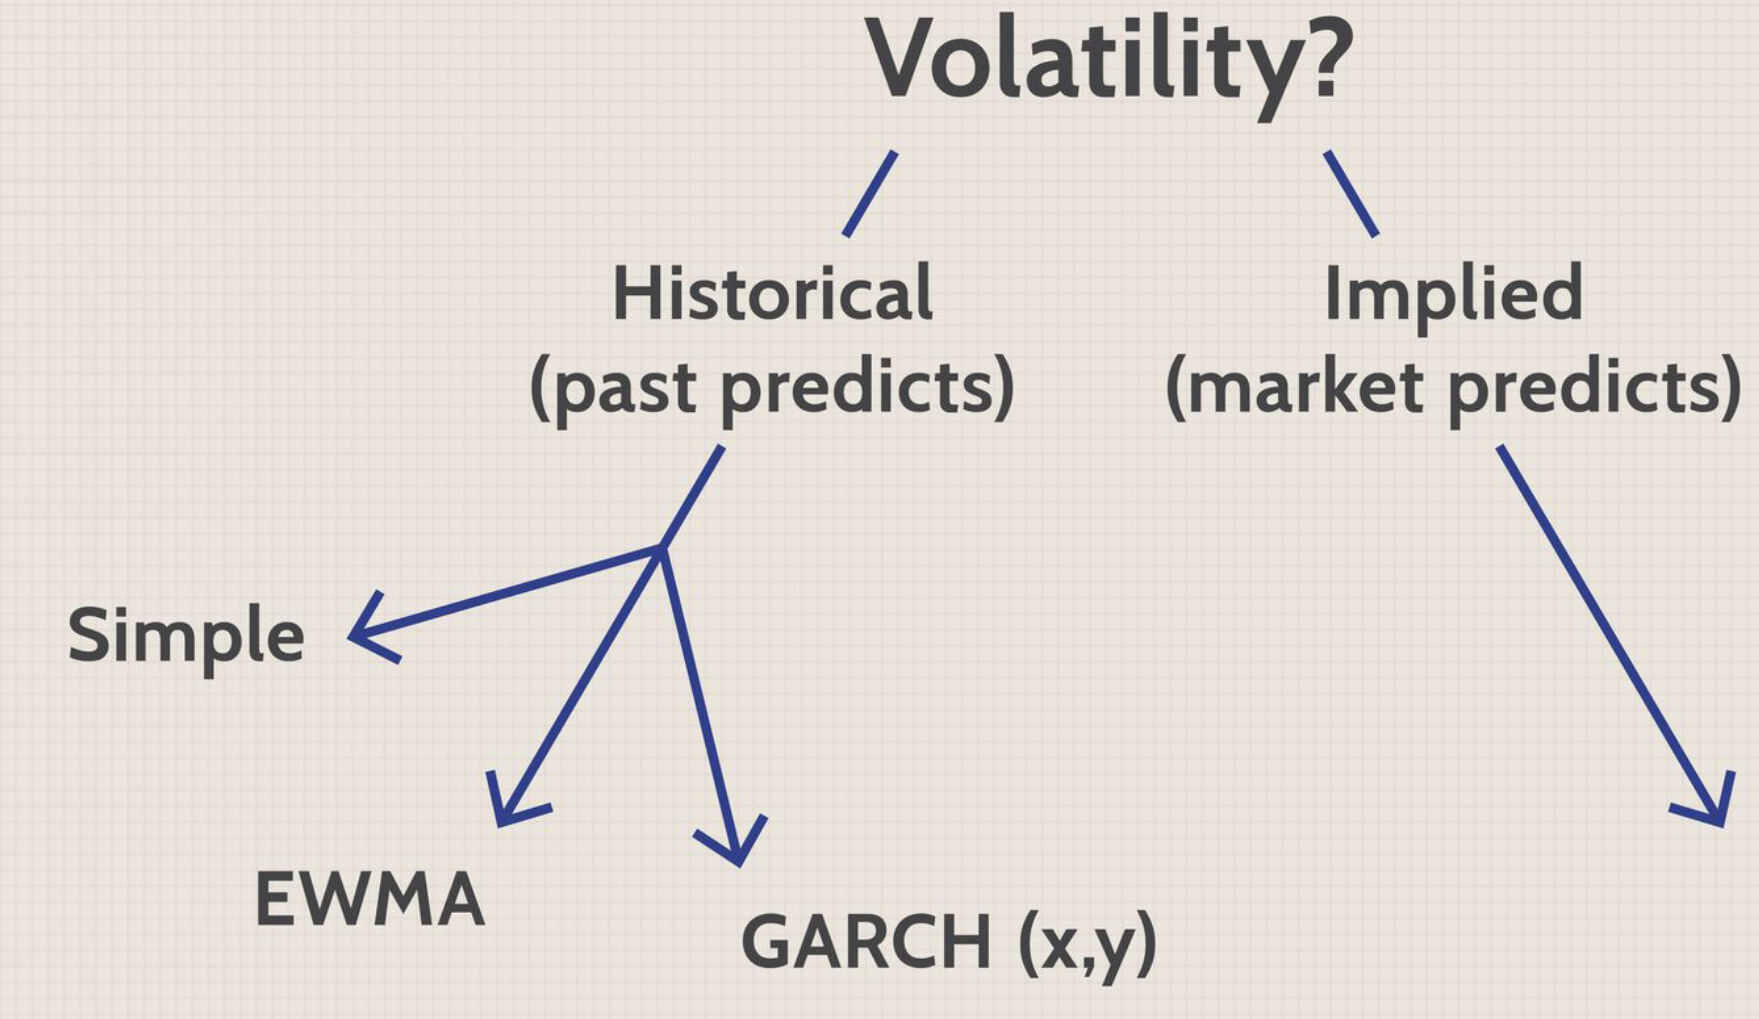
\includegraphics[width=0.75\paperwidth]{../static/course_3_img/volatility_decision_tree.PNG}}
  \hspace*{15pt}\hbox{\scriptsize Credit:\thinspace{\scriptsize\itshape Sabrina Jiang}}          
  
\end{frame}

\begin{frame}
  \frametitle{EWMA Model}
  \makebox[\linewidth]{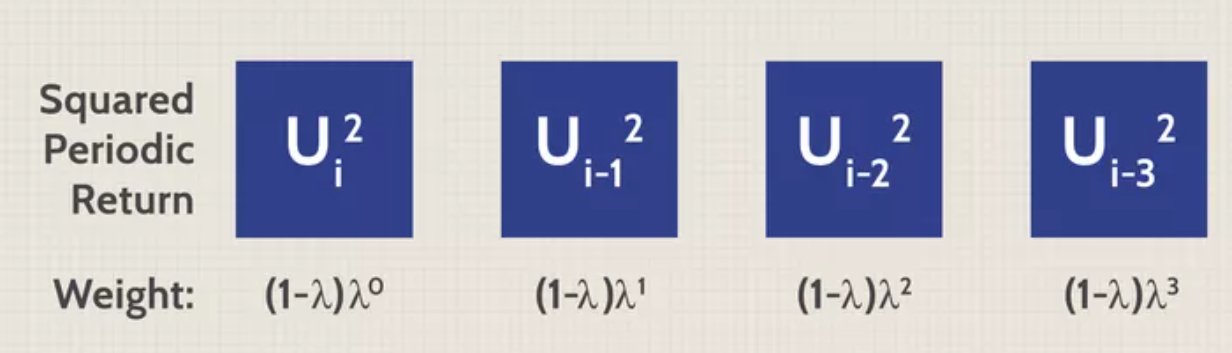
\includegraphics[height=0.35\paperheight]{../static/course_3_img/ewma_squared_returns.PNG}}
  \hspace*{15pt}\hbox{\scriptsize Credit:\thinspace{\scriptsize\itshape Sabrina Jiang}}          

  \medskip

  \makebox[\linewidth]{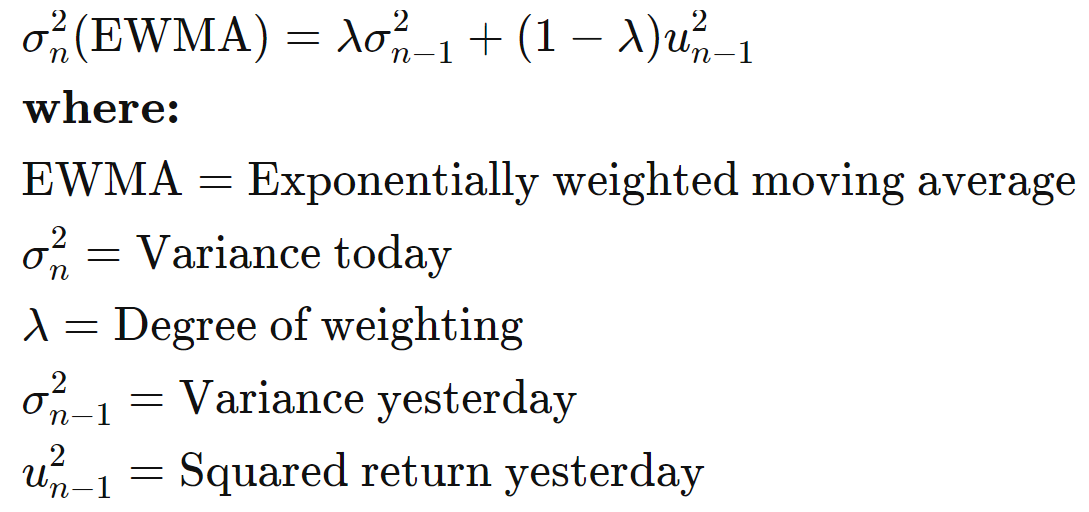
\includegraphics[height=0.35\paperheight]{../static/course_3_img/ewma_formula.PNG}}
  %\hspace*{15pt}\hbox{\scriptsize Credit:\thinspace{\scriptsize\itshape Sabrina Jiang}}          
  
\end{frame}


\begin{frame}
  \frametitle{EWMA Weights}
  \makebox[\linewidth]{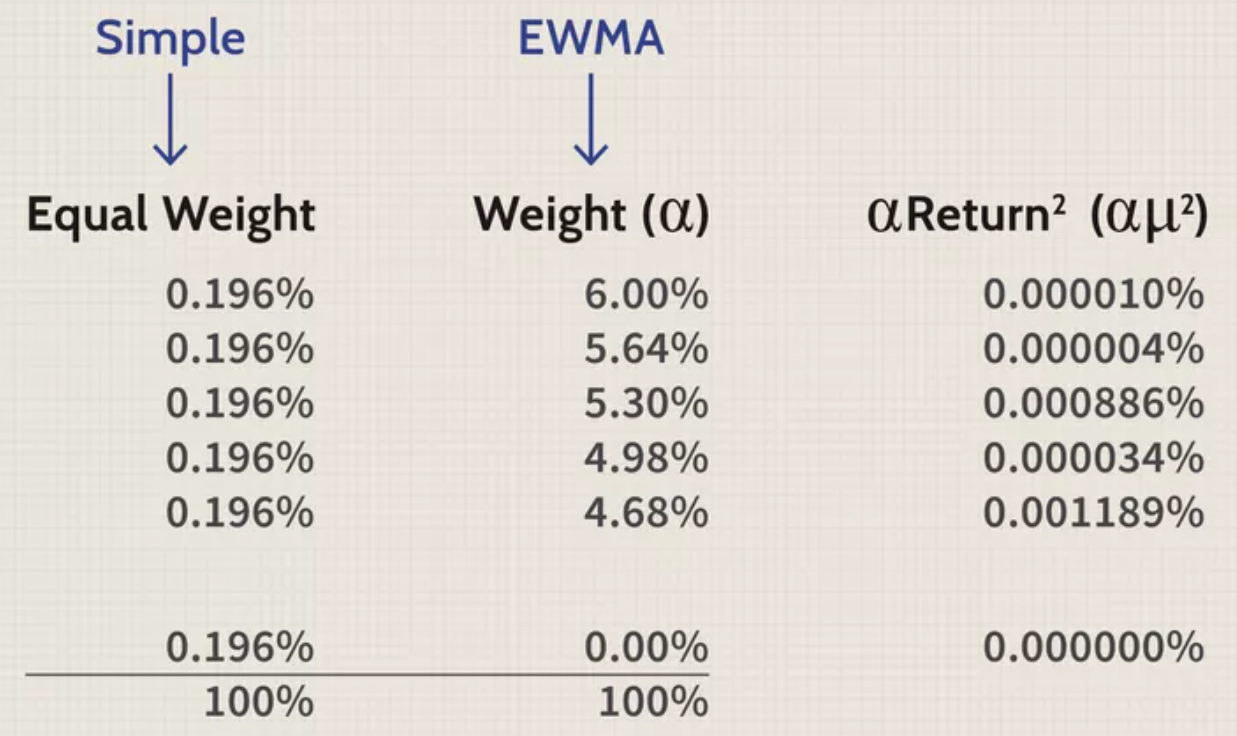
\includegraphics[height=0.65\paperheight]{../static/course_3_img/ewma_weights.PNG}}
  %\hspace*{15pt}\hbox{\scriptsize Credit:\thinspace{\scriptsize\itshape Sabrina Jiang}}            
\end{frame}


\begin{frame}
  \frametitle{Homoscedasticity and Heteroscedasticity}
  \makebox[\linewidth]{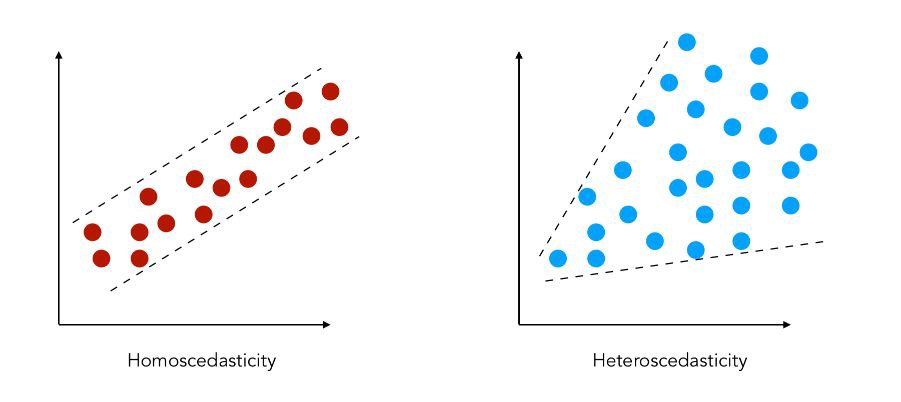
\includegraphics[width=0.95\paperwidth]{../static/course_3_img/homo_hsk.jpeg}}
  \hspace*{15pt}\hbox{\scriptsize Credit:\thinspace{\scriptsize\itshape Medium.com}}          
\end{frame}

\begin{frame}
  \frametitle{GARCH Models}

  \begin{alertblock}{Meaning}
    \textbf{GARCH}: \textbf{G}eneralized \textbf{A}uto\textbf{R}egressive \textbf{C}onditional \textbf{H}eteroscedasticity    \    
  \end{alertblock}

\medskip
  
\emph{Reference: Bollerslev, T. (1986), Generalized Autoregressive Conditional Heteroskedasticity. Journal of
  Econometrics, 31, 307-327}\\

\end{frame}


\begin{frame}
\begin{block}{Definition: GARCH Model}

  The stochastic process $\{ \epsilon_t, \ t \ in \mathbb{Z} \}$ is said to be a \textbf{GARCH}(p,q) process if:

  \begin{equation*}
    \epsilon_t = Z_t \sigma_t
  \end{equation*}

  \medskip

  where $Z_t$ is a sequence of i.i.d variables with $\mathbb{E}(Z_t) = 0$ and $\mathbb{V}(Z_t) = 1$, and $\sigma_t$ is a non-negative process such that:
  \begin{equation*}
    \sigma^2_t = \omega + \sum^p_{i=1} \alpha_i \epsilon^2_{t-i} + \sum^p_{i=1} \beta_i \sigma^2_{t-i}
  \end{equation*}

  \medskip

  with $\omega >0$, $\forall \ i, (\alpha_i, \beta_i) \ \in \ \mathbb{R}^{+,2}$ and $\sum^p_{i=1} \alpha_i + \sum^p_{i=1} \beta_i <1$  
\end{block}
\end{frame}


\begin{frame}
  \frametitle{GARCH: Intuition}
  \begin{wideitemize}
  \item The conditional variance of a GARCH(p, q) depends on:
    \begin{itemize}
    \item The first p lag of the $\epsilon_t^2$ (e.g. the squared error terms)
    \item The first $q$ lag of the conditional variance $\sigma^2$
    \end{itemize}

 \begin{equation*}
    \sigma^2_t = \omega + \underbrace{\sum^p_{i=1} \alpha_i \epsilon^2_{t-i}}_{\text{ARCH Components}} + \underbrace{\sum^p_{i=1} \beta_i \sigma^2_{t-i}}_{GARCH components}
  \end{equation*}
    
   
  \item The parameters $\alpha_i$ are often called the \textbf{ARCH parameters}
  \item The parameters $\beta_i$ are often called the \textbf{GARCH parameters}
\end{wideitemize}
  
\end{frame}

\begin{frame}
  \frametitle{GARCH(1, 1)}

  \begin{alertblock}{Tip}
GARCH(1,1) specifications are generally sufficient to capture the dynamics of the conditional variance
  \end{alertblock}

  \medskip
  
\begin{block}{Special Case: GARCH(1, 1)}

  The stochastic process $\{ \epsilon_t, \ t \ in \mathbb{Z} \}$ is said to be a \textbf{GARCH}(1,2) process if:

  \begin{equation*}
    \epsilon_t = Z_t \sigma_t
  \end{equation*}

  \medskip

  where $Z_t$ is a sequence of i.i.d variables with $\mathbb{E}(Z_t) = 0$ and $\mathbb{V}(Z_t) = 1$, and $\sigma_t$ is a non-negative process such that:
  \begin{equation*}
    \sigma^2_t = \omega + \alpha \epsilon^2_{t-1} + \beta \sigma^2_{t-1}
  \end{equation*}

  \medskip

  with $\omega >0$, $\alpha \geq 0, \beta \geq 0$ and $\alpha + \beta <1$  
\end{block}
\end{frame}


\begin{frame}
  \frametitle{Conditional Variance Persistences: Intrinsic and Extrinsic}
  \begin{itemize}
  \item The conditional variance $\sigma_t^2 = \omega + \alpha \epsilon^2_{t-1} + \beta \sigma^2_{t-1}$ depends on two effects:
    \begin{itemize}
    \item An \textbf{intrinsic persistence} effect through the first lag of the conditional variance
    \item An \textbf{extrinsic persistence} effect
    \end{itemize}
    
  \item Following a positive (or negative) shock at time \emph{t-1}, the conditional variance at time \emph{t} increases (impact effect) and thus it has an impact on $\epsilon_t = Z_t \sigma_t$

    \begin{equation*}
      \text{shock} \ z_{t-1} \ > \ 0 \Rightarrow \ \epsilon_{t-1} \ \uparrow \ \Rightarrow \ \sigma_t \ \uparrow \ \dots
    \end{equation*}

  \item Starting from the next period (at time $t$), the effect of the shock at $t-1$ on the conditional variance at $t+1$ passes through the conditional variance at time $t$ (intrisic persistence)

    \begin{equation*}
      \text{shock} \ z_{t-1} \ \Rightarrow \ \sigma_t \ \uparrow \ \Rightarrow \ \sigma^2_{t+1} \ \uparrow 
    \end{equation*}
\item The overall effect of a shock can be decomposed into a \textbf{contemporaneous effect}, which depends on $\alpha$ and a \textbf{persistence effect} that depends on $\beta$
    
  \end{itemize}
\end{frame}



\begin{frame}
  \frametitle{Remarks}

  \begin{wideitemize}
  \item It is often the case that:
      \begin{wideenumerate}
  \item The sum of the estimates of $\alpha$ and $\beta$ are generally close (but below 1)
  \item The estimate of $\beta$ is generally greater than the one of $\alpha$
  \item The estimate of $\beta$ is generally larger than 0.90 for daily returns and the estimate of $\alpha$ is below 0.1
  \end{wideenumerate}
  \item Be careful: it is not a general rule, just an observation.
  \end{wideitemize}  
\end{frame}

\begin{frame}
  \frametitle{GARCH Extensions}
  \begin{wideitemize}
  \item I won't cover them during the course but many extensions have been proposed to extend the GARCH model, including model for dealing with \textbf{asymmetric responses}, \textbf{persistence} and \textbf{long-memory}
    \begin{wideitemize}
      \item \textbf{IGARCH model}: Integrated GARCH (model persistence)
      \item \textbf{GARCH-M model}: GARCH mean, when the mean depends on the volatility
      \item \textbf{GJR-GARCH model}: Glosten, Jagannathan and Runkle (1993): asymmetric with non-linearities
      \item \textbf{TGARCH model}: Threshold GARCH captures regimes change
      \item \textbf{EGARCH model}: Exponential GARCH captures asymmetric responses and big shocks
    \end{wideitemize}
  \end{wideitemize}
\end{frame}

\section{Distributional Forecasts and Prediction Intervals}
\begin{frame}{From Point Forecasts to Distributional Forecasts}

  \begin{wideitemize}
    \item A forecast $\hat{y}_{T+h|T}$ is (usually) the mean of the conditional distribution: $Y_{T+h} | Y_1, \dots Y_T$
    \item Most models produces Gaussian distributed forecast
    \item Because models assumes Gaussian residuals: remember that the residuals are the stochastic components that are determining the distribution of both the estimators and the forecasts
    \item The forecast distribution describes the probability to forecast any future value
  \end{wideitemize}

  %TODO: add a chart
    
\end{frame}


\begin{frame}{Distributional Forecasts}

  Assuming the \textbf{residuals are uncorrelated} with variance $\sigma^2$, and with an estimate $\hat{\sigma^2}$

  \begin{alertblock}{Model Typology}
    \begin{wideitemize}
      \item \textbf{Mean:} $Y_{T+h|T} = \mathcal{N}(\overline{Y}, (1+\frac{1}{T})\hat{\sigma^2})$
      \item \textbf{Naive:} $Y_{T+h|T} = \mathcal{N}(Y_T, h\hat{\sigma^2})$
      \item \textbf{Seasonal Naive:} $Y_{T+h|T} = \mathcal{N}(Y_{T+h-m(k+1)}, (k+1)\hat{\sigma^2})$
      \item \textbf{Drift:} $Y_{T+h|T} = \mathcal{N}(Y_{T} +\frac{h}{T-1}(Y_T - Y_1), h\frac{T+h}{T}\hat{\sigma^2})$
    \end{wideitemize}
  \end{alertblock}

\medskip

\begin{wideitemize}
  \item where $k$ is the integer part of $\frac{h-1}{m}$
  \item Note that when $h=1$ and $T$ is large, these all give the same approximate variance $\hat{\sigma^2}$
\end{wideitemize}

\end{frame}



\begin{frame}{Prediction Intervals}
  \begin{block}{Definition}
      A prediction interval gives \textbf{a region} within which we expect $Y_{T+h}$ to lie with \textbf{a specified probability}
  \end{block}

\medskip
  
  \begin{wideitemize}
  \item Assuming that the forecasting errors are normally distributed, then a 95\% prediction interval is:
    \begin{equation*}
      Y_{T+h|T} \pm 1.96 \hat{\sigma_h}
    \end{equation*}
  \item where $\hat{\sigma_h}$ is the standard deviation of the h-step distribution
  \item when $h=1$, $\hat{\sigma_h}$ can be estimated from the residuals  
  \end{wideitemize}  
\end{frame}


\begin{frame}
  \frametitle{Prediction Interval Fit}
     \makebox[\linewidth]{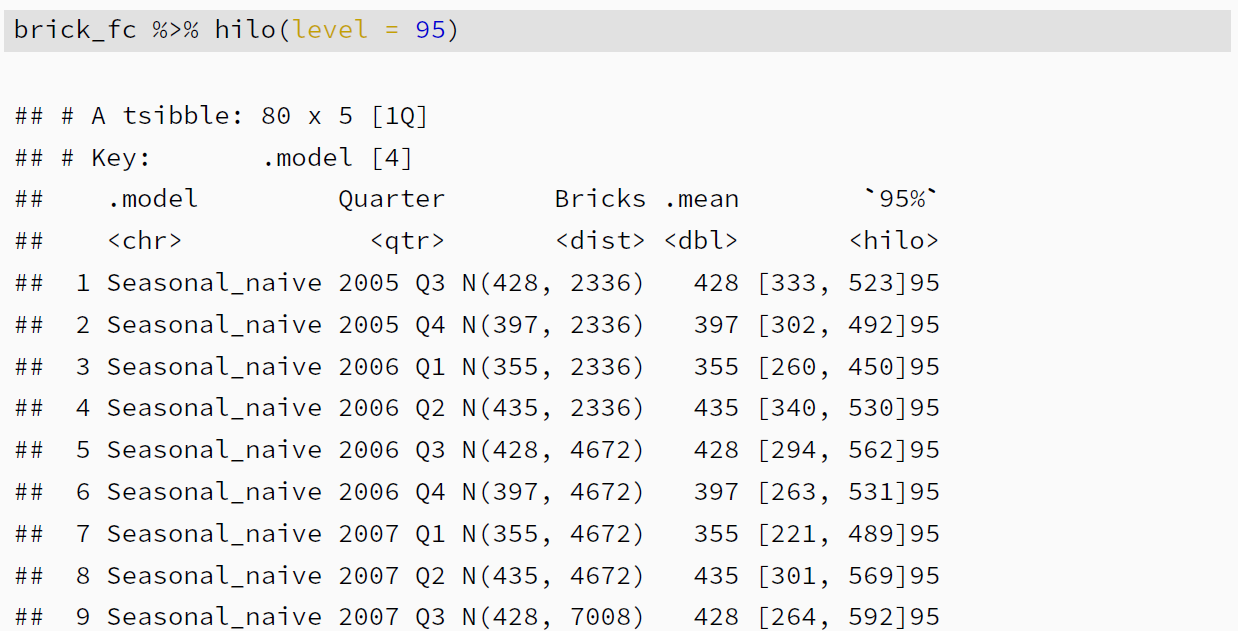
\includegraphics[width=0.95\paperwidth]{../static/course_3_img/prediction_interval.PNG}}  
\end{frame}


\begin{frame}{Why Prediction Intervals Matter}
  \begin{wideitemize}
    \item \textbf{Point forecasts are often useless without a measure of uncertainty} (such as prediction intervals)
    \item Prediction intervals require a \textbf{stochastic model} (with random errors, etc.)
    \item For most models, prediction intervals get wider as the forecast horizon increases
    \item The degree of confidence (the probability) impacts the width of the prediction interval
    \item Usually too narrow due to unaccounted uncertainty: pay attention
  \end{wideitemize}  
\end{frame}


\begin{frame}
  \frametitle{Difference between Confidence Interval and Prediction Interval}
  \begin{wideitemize}


 \item A confidence interval informs about where the true parameter of a model can be
   \begin{itemize}
     \item \textbf{Confidence interval quantifies the uncertainty about the model}, or the distance between the model and reality
     \item Confidence interval are associated with a wide range of parameters, values, etc.
     \item They inform about how the model represents well the reality
     \item Wide confidence intervals are associated with a less accurate model, and/or a very volatile model
   \end{itemize}

    
  \item The prediction interval predicts in what range a future individual observation will fall
    \begin{itemize}
      \item \textbf{Prediction interval quantifies the uncertainty about the future}, or the distance between today and the future
      \item Prediction interval are not about the parameters of the model, but about the dependent variable ($y_t$)
      \item The problem is that prediction intervals tend to neglect the uncertainty about the parameters used to generate the forecasts...
    \end{itemize}   
  \end{wideitemize}
  
\end{frame}


\begin{frame}
  \frametitle{Difference between Confidence Interval and Prediction Interval}
     \makebox[\linewidth]{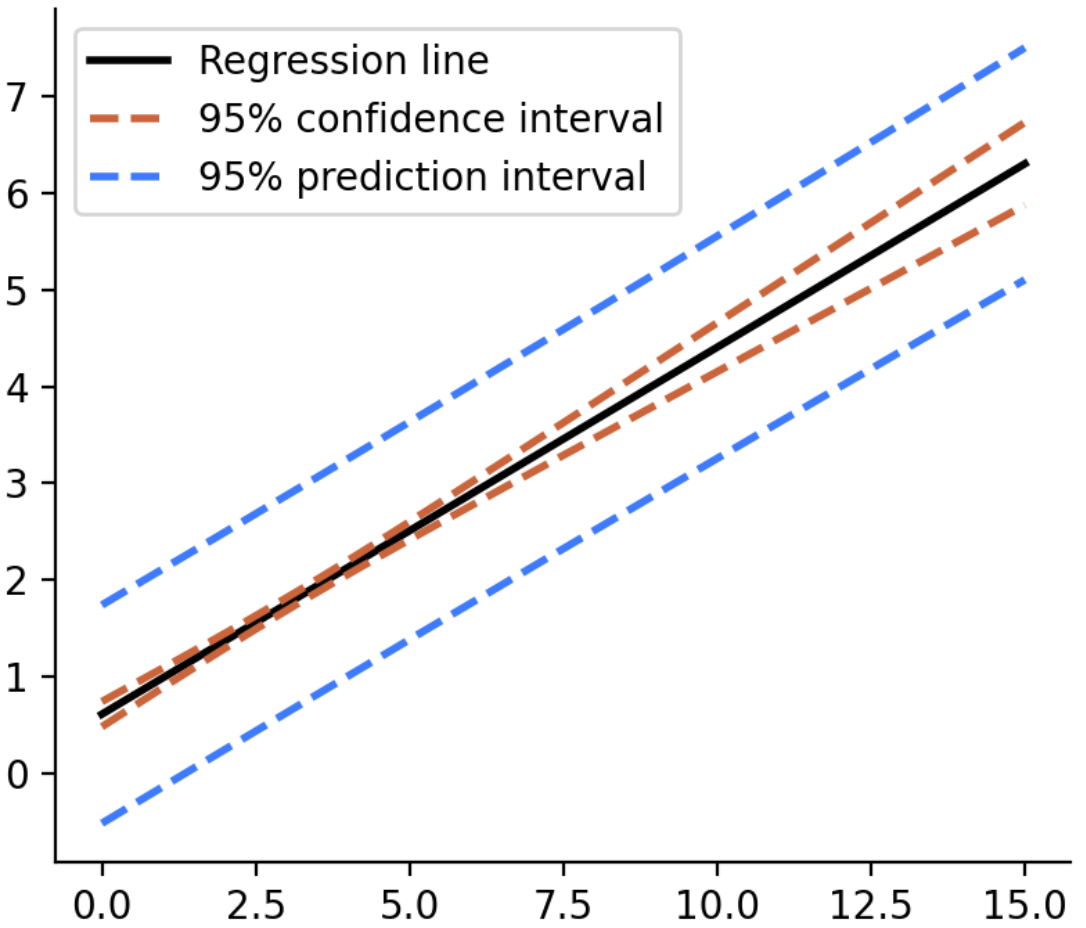
\includegraphics[width=0.75\paperwidth]{../static/course_3_img/pi_ci.png}}  
\end{frame}




\end{document}